\documentclass[a4paper,german,12pt,smallheadings]{scrartcl}
\usepackage[T1]{fontenc}
\usepackage[utf8]{inputenc}
\usepackage{babel}
\usepackage{tikz}
\usepackage{wrapfig}
\usepackage{enumerate}
\usepackage{amsmath}
\usetikzlibrary{calc,intersections,through,backgrounds}
\begin{document}

\section*{Gruppenstruktur eines Kreises}
\begin{wrapfigure}{r}{0pt}
  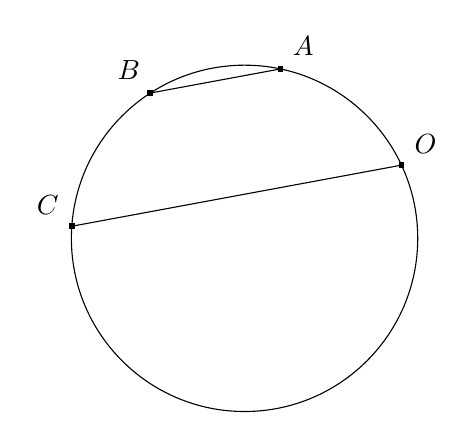
\begin{tikzpicture}
    \pgfmathsetmacro{\radius}{2.2}
    \pgfmathsetmacro{\zeroAngle}{25}
    \pgfmathsetmacro{\aAngle}{53}
    \pgfmathsetmacro{\bAngle}{98}
    \pgfmathsetmacro{\cAngle}{\aAngle + \bAngle}

    \coordinate (O) at (\zeroAngle:\radius);
    \coordinate (A) at (\zeroAngle + \aAngle:\radius);
    \coordinate (B) at (\zeroAngle + \bAngle:\radius);
    \coordinate (C) at (\zeroAngle + \cAngle:\radius);

    \node (S) [name path=S,draw,circle through=(O)] at (0,0) {};

    \node [fill=black,inner sep=1pt,label=\zeroAngle:$O$] at (O) {};
    \node [fill=black,inner sep=1pt,label=\aAngle:$A$] at (A) {};
    \node [fill=black,inner sep=1pt,label=\bAngle:$B$] at (B) {};
    \node [fill=black,inner sep=1pt,label=\cAngle:$C$] at (C) {};
    \draw (A) -- (B);
    \draw (O) -- (C);
  \end{tikzpicture}
\end{wrapfigure}

Gegeben sei ein Kreis mit beliebigem Radius. Auf diesem Kreis befinde sich ein
fester Punkt $O$. Gegeben seien außerdem zwei weitere beliebige Punkte auf dem
Kreis, die wir $A$ und $B$ nennen.

\noindent Die Multiplikation $C = A \cdot B$ sei durch folgendes geometrisches Verfahren
definiert:

\begin{enumerate}
  \item Ziehe eine Gerade durch $A$ und $B$ um $\overline{AB}$ zu erhalten.
  \item Konstruiere eine Gerade durch $O$, parallel zu $\overline{AB}$. Der
    Schnittpunkt mit dem Kreis ergibt den Punkt $C$.
\end{enumerate}

\noindent Aufgaben:

\begin{enumerate}[a)]
  \item Begründe, dass die Multiplikation symmetrisch ist ($A \cdot B = B \cdot A$)
  \item Was ist das neutrale Element dieser Multiplikation?
  \item Was ist das inverse Element dieser Multiplikation?
  \item Ist die Multiplikation assoziativ?
  \item Schließe, dass $(\text{Kreis}, \cdot)$ eine Gruppe definiert.
\end{enumerate}

%\noindent \textit{Hinweis}: Komplexe Zahlen

\end{document}
